\subsubsection{Tyk}
\label{soa:tecnologias:tyk}

Tyk es un API Gateway liviano y plataforma de administración, todo en un mismo producto, que permite controlar quién tiene acceso a la API, cuándo y cómo.  Está escrito en Go, es sencillo de configurar, y sus únicas dependencias son Redis y MongoDB (\texttt{v2.6} o superior, utilizado para el almacenamiento de los datos de acceso, de caracter opcional).

El API Gateway de Tyk se implementa delante de nuestras \glspl{acro:api} para gestionar la autorización, el control de acceso y la limitación de acceso a nuetros servicios (\eng{rate limiting}).  De esta manera permite concentranos en el desarrollo de servicios para nuestras \glspl{acro:api}, en lugar de implementar herramientas para la administración de la infraestructura.  Esto nos permite enfocarnos en el desarrollo de los servicios, para luego integrarlos fácilmente al API Gateway.

Tyk posee un portal para desarrolladores que permite analizar quién y cómo utiliza nuestras \glspl{acro:api}, limitar el acceso a los servicios (\eng{rate limiting}), modificar parámetros de \eng{caching}, y generar o revocar una \eng{API Key}, entre otras características.  Todo esto de manera muy sencilla y centralizada, evitando trasladar parte de esta funcionalidad a los servicios.

\paragraph{Licencia}

Tyk se encuentra publicado bajo licencia Mozilla Public License Version 2.0\footnote{La misma puede ser consultada en \url{https://www.mozilla.org/en-US/MPL/2.0}}.

\paragraph{Características principales}

A continuación presentamos un breve listado de las características principales que Tyk ofrece actualmente:

\begin{itemize}
  \item RESTful API: provee una \gls{acro:api} RESTful para configurar Tyk mediante peticiones a ésta.
  \item Múltiples protocolos de acceso: Tyk soporta múltiples métodos de acceso a la \gls{acro:api}:
  \begin{itemize}
    \item \textbf{Token-based:} autenticación mediante una clave de \gls{acro:api}. \\
    \url{https://tyk.io/v1.9/access-control/access-keys}
    \item \textbf{HMAC:} permite autenticar la identidad del cliente (\eng{consumer}) mediante firmas \gls{acro:hmac} en los mensajes. \\
    \url{https://tyk.io/v1.9/access-control/hmac}
    \item \textbf{Basic Auth:} autenticación mediante usuario y contraseña. \\
    \url{https://tyk.io/v1.9/access-control/basic-auth}
    \item \textbf{OAuth2:} autenticación mediante el protocolo OAuth 2.0. \\
    \url{https://tyk.io/v1.9/access-control/oauth2}
    \item \textbf{JSON Web Token:} provee autenticación mediante el uso del estándar JSON Web Tokens. \\
    \url{https://tyk.io/v1.9/access-control/json-web-tokens}
    \item \textbf{Keyless:} provee acceso abierto, sin restricciones. \\
    \url{https://tyk.io/v1.9/access-control/keyless}
  \end{itemize}

  \item Rate Limiting: permite configurar fácilmente el \eng{rate limit} para cada \eng{API Key}, definiendo la cantidad de peticiones por segundo y el tiempo de expiración (1 hora, 6 horas, 12 horas, 24 horas, 1 semana, 1 mes o que nunca expire). \\
  \url{https://tyk.io/v1.9/quotas-limits-security/access-control}
  \item Policies: habilita a crear políticas para aplicar \eng{quotas}, \eng{rate limit} y \eng{access rights} a un conjunto de claves de acceso. \\
  \url{https://tyk.io/v1.9/quotas-limits-security/limiting-access}
  \item Permisos por \eng{endpoint} (\eng{Path by path permissions}): permite configurar permisos de acceso para cada \eng{endpoint}.
  \item Expiración de claves de acceso (\eng{Key Expiry}): admite el control del tiempo de expiración de una clave de acceso. \\
  \url{https://tyk.io/v1.9/rest-api/api-key-management}
  \item Versionado de las \glspl{acro:api}: permite versionar las \glspl{acro:api} de tres maneras diferentes:
  \begin{itemize}
    \item Mediante una clave en el encabezado \gls{proto:http}, por ejemplo \texttt{X-Api-Version}.
    \item Por \gls{acro:url} o parámetro en el cuerpo de la petición.
    \item Por el primer elemento de una \gls{acro:url}, ejemplo \texttt{/v1/resource/id} (donde \texttt{v1} es la versión).
  \end{itemize}
  \url{https://tyk.io/v1.9/api-management/api-versioning}
  \item Analíticas: registro detallado de los accesos a las \glspl{acro:api}.
  \item Zero downtime restarts: las configuraciones de Tyk pueden realizarse dinámicamente, reiniciar los servicios sin que esto afecte los requerimientos activos.
  \item Web Hooks: fácilmente se pueden integrar notificaciones y eventos que permitirán mejorar el monitoreo.
  \item Lista blanca de IPs: acceso autorizado únicamente a las direcciones IP indicadas en la lista blanca.
  \item Límite de tamaño: permite limitar el tamaño de las peticiones que llegan a las \gls{acro:api}, evitando que los sevicios sean saturados por peticiones.
  \item Health checks: provee verificación del estado de los nodos.
  \item Mock \glspl{acro:api}: permite crear \glspl{acro:api} de prueba, muy útil para el desarrollo de nuevos servicios.
  \item Soporte para API Blueprint: permite importar rápidamente una \gls{acro:api} en formato \gls{lang:json}.
  \item Soporte para Swagger: permite importar archivos que respeten \nameref{soa:tecnologias:openapi-spec} (anteriormente conocida como \eng{The Swagger specification}).
  \item Transformaciones de solicitudes y respuestas: permite utilizar templates para transformar datos y agregar o quitar cabeceras \textit{al vuelo}.
  \item Caching: permite implementar una cache para las respuestas por \eng{endpoint} o globalmente, incrementando la velocidad de respuesta, al mismo tiempo que se disminuye la carga de las \gls{acro:api}. \\
  \url{https://tyk.io/v1.9/api-management/caching}
  \item Documentación de la API: el portal de Tyk soporta API Blueprint y Swagger.
  \item Endpoints virtuales: como AWS Lambda Functions\footnote{Cf. \url{https://aws.amazon.com/es/lambda/details}}, permite correr fragmentos de JavaScript en los \eng{endpoints} para manejar interacciones complejas de servicios, tales como solicitud de procesamiento por lotes. \\
  \url{https://tyk.io/v1.9/api-management/virtual-endpoints}
  \item Foco en microservicios: permite implementar el patrón \eng{circuit breaker}, \eng{hard timeouts} y \eng{round robin}, para balancear la carga en el acceso a los servicios. \\
  \url{https://tyk.io/v1.9/api-management/circuit-breakers} \\
  \url{https://tyk.io/v1.9/api-management/load-balancing}
  \item Uptime Awareness: Tyk activamente monitorea los \eng{endpoints} de las \glspl{acro:api} y notifica cuando alguno de estos se encuentra fuera de servicio. \\
  \url{https://tyk.io/v1.9/uptime-tests/uptime-tests}
\end{itemize}

\paragraph{Instalación y prueba}

A continuación se detallan los pasos necesarios para la instalación y ejecución de Tyk, basándonos en su documentación oficial \footnote{\url{https://tyk.io}}.

Tyk puede instalarse de varias maneras:

\begin{itemize}
  \item Instalar Tyk en Ubuntu desde paquetes.
  \item Instalar Tyk en Redhat o CentOS usando paquetes RPM.
  \item Instalar Tyk desde una imagen Docker.
\end{itemize}

En nuestro caso particular se optó por instalar Tyk en Ubuntu 14.04 desde paquetes, a continuación desarrollaremos esta forma de instalación.

Pre-requisitos:\\
Asegurarse que el puerto \texttt{8080} esté abierto: este puerto es utlizado por el API Gateway.\\
Asegurarse que el puerto \texttt{3000} esté abierto: este puerto es utlizado por el dashboard, quien provee la GUI y el portal para desarrolladores.

Primero preparamos el ambiente del equipo para obtener los paquetes a instalar:

\begin{listing}[H]
  \bashfile{src/03-capitulo-3/tecnologias/nodo-central/code/tyk/00-preparacion.sh}
  \caption{Preparación del servidor para instalar Tyk}
  \label{soa:tecnologias:tyk:bash-preparacion}
\end{listing}

Luego, procedemos a instalar Tyk y sus dependencias:

\begin{listing}[H]
  \bashfile{src/03-capitulo-3/tecnologias/nodo-central/code/tyk/01-instalacion.sh}
  \caption{Instalación y arranque de Tyk}
  \label{soa:tecnologias:tyk:bash-instalacion}
\end{listing}


\paragraph{Integración con nuestro diseño}

Para el nuevo diseño de la arquitectura, se implementaría el API Gateway de Tyk como un nodo central, en el cual se enrutarían todas las peticiones realizadas desde los diferentes clientes.  Detrás de Tyk tendríamos replicadas distintas instancias de las \glspl{acro:api}, las cuales nos permitirían escalar horizontalmente de forma sencilla, ya que Tyk se encargaría de realizar el balanceo de la carga a cualquiera de estas instancias replicadas.

La migración de la vieja nube a la nueva arquitectura se iría realizando de manera progresiva, cambiando la lógica de acceso antigua por la nueva en cada aplicación.  De esta manera tendríamos conviviendo al mismo tiempo la vieja nube y la nueva arquitectura que en el presente trabajo estamos definiendo.

\begin{figure}[H]
  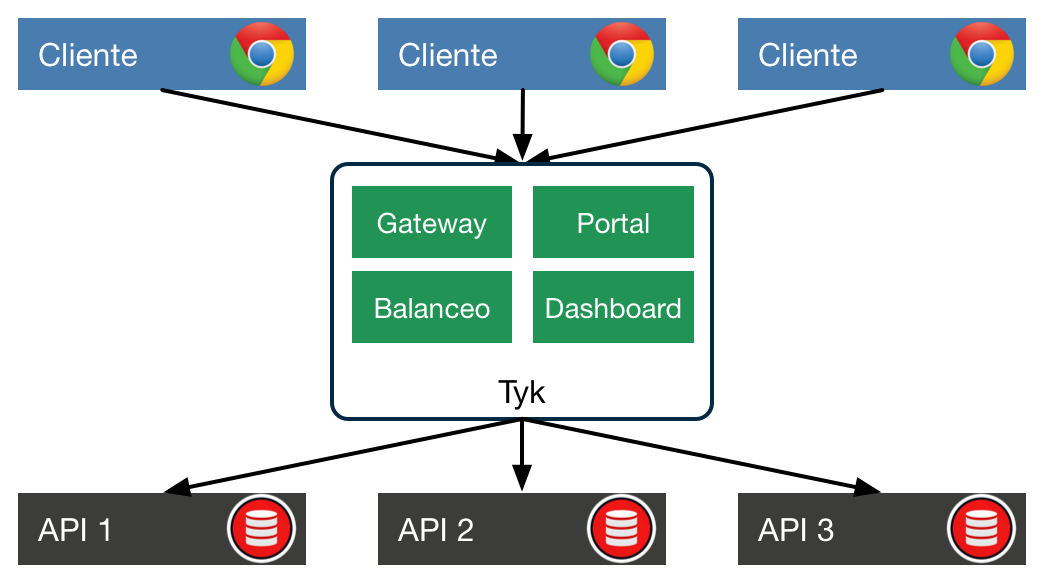
\includegraphics[width=\linewidth]{src/images/03-capitulo-3/tecnologias/tyk/tyk-integracion-arquitectura.png}
  \caption{Esquema de integración de Tyk en nuestra propuesta}
  \label{fig:integracion-tyk-arquitectura}
\end{figure}
